\section{Proposed Method}

In this section, we formalize the task of building a confidence region in the Entropy-Complexity manifold.
Then, we present our proposal to change space through the algorithm of the principal components analysis.
Our goal is to find a latent space representative of the data, without the restrictions of a curvilinear space.
Through this new representation of the data, we calculate empirical regions with different levels of confidence.
Finally, after calculating these regions, we build a test statistic that determines the probability that a given sequence belongs to the distribution of the points provided.

%\subsection{Problem Formalization}

\subsection{Overall Framework}

The structure of our proposal is shown in Fig.~\ref{fig:methodology}. 
It consists of two steps:
\begin{itemize}
    \item \textbf{Empirical confidence region}: With the data present in a Euclidean plane, we can easily calculate empirical regions that involve the data with a certain level of confidence.
    \item \textbf{Construction of a test statistic}: To measure the similarity of new data sequences with the empirical points, a test statistic was proposed. 
    By acquiring a p-value less than 0.5, we can reject the null hypothesis, which states that such data belong to the empirical probability distribution used for the construction of the confidence region.
\end{itemize}

\begin{figure}[H]
    \centering
    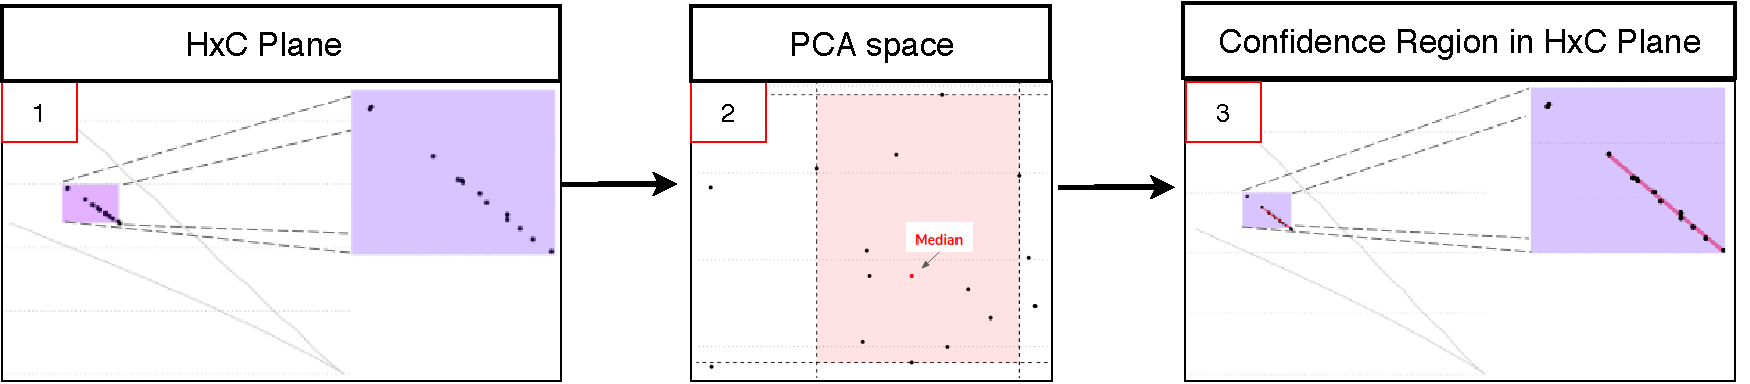
\includegraphics[width=\linewidth]{Figures/Methodology.pdf}
    \caption{Outline of the methodology used for the construction of confidence regions.}
    \label{fig:methodology}
\end{figure}


\subsection{Empirical Confidence Regions}\label{confidenceRegions}

As we do not know the joint probability distribution of the pair $(h, c)$ for a sequence of random variables collectively independent and identically distributed according to a uniform law, studies involving classical bi-variate analysis, linear regression, and generalized linear models become unfeasible.
Therefore, for the construction of our proposal, we adopted a non-parametric approach, making an empirical analysis of data obtained from physical sources and using them as our reference in the search for confidence regions.

The set of all feasible pairs in the $H \times C$ plane is found in a compact subset of $\mathbbm{R}^2$, which has limits with explicit expressions for the boundaries of this closed manifold, dependent only on the dimension of the probability space considered, that is $D!$ in the traditional Bandt-Pompe method~\cite{martin2006generalized}.
Due to such quotas, some limitations are generated, such as the absence of a representative distance metric and the difficulty of proposing confidence regions.
In view of this, it is necessary to apply an orthogonal projection in the data for a new two-dimensional coordinate system to solve these restrictions.
A classic proposal in these categories of problems is the principal component analysis algorithm~\cite{wold1987principal}.

Let ${\mathcal P} = \{p_n\}_{n = 1}^{N}$ be a set of $N$ observations in the $H \times C$ plane, where ${p_n} = (h_n, c_n)$ corresponds to a time series.
We propose in this work the use of a latent space $\Omega_1 \times \Omega_2$ obtained by the PCA for the construction of empirical confidence regions, which hereinafter referred to we call HC-PCA regions.
Let $\{(u_n, v_n)\}_{n = 1}^N$ uncorrelated observations obtained by the representation of ${\mathcal P}$ in the latent space $\Omega_1 \times \Omega_2$.
For simplicity, and without loss of generality, assume $N$ odd; 
in the proposed methodology, we find a parallelepiped that contains \SI{100}{\minusalphapercent} of the points in the $H \times C$ plane with the following steps:
%We apply a principal component analysis to these points and obtain $\{(u_n,v_n)\}_{n=1}^N$.
%This transformation yields uncorrelated observations in the $\Omega_1\times\Omega_2$ plane.
%We will find the empirical confidence regions on the $\Omega_1\times\Omega_2$ plane, and then they will be mapped back to the $H \times C$ plane.
\begin{enumerate}
    \item Find the ranks that sort the values of the first principal component $\bm u=(u_1,u_2,\dots,u_N)$ in ascending order: $\bm r=(r_1,r_2,\dots,r_N)$, i.e., $u_{r_1}$ is the minimum value, and $u_{r_N}$ is the maximum value.
    \item Find point $(u,v)$ whose first principal component is the median: $(u_{r_{(N+1)/2}}, \cdot)$.
    \item Find the point $(u,v)$ whose first principal component is the quantile $\alpha/2$: $(u_{r_{[N\alpha/2]}}, \cdot)$.
    \item Find the point $(u,v)$ whose first principal component is the quantile $1-\alpha/2$: $(u_{r_{[N(1-\alpha/2)]}}, \cdot)$.
    \item The values $u_{r_{[N\alpha/2]}}$ and $u_{r_{[N(1-\alpha/2)]}}$ are the rightmost and leftmost bounds of the box, respectively.
    \item The top and bottom bounds of the box are the minimum and maximum values of the second principal component of the points whose first principal component is at least $u_{r_{[N\alpha/2]}}$ and at most $u_{r_{[N(1-\alpha/2)]}}$; denote these values $v_{\min}$ and $v_{\max}$, respectively.
    \item The corners of the box are 
    $(u_{r_{[N\alpha/2]}}, v_{\min})$, 
    $(u_{r_{[N\alpha/2]}}, v_{\max})$, 
    $(u_{r_{[N(1-\alpha/2)]}}, v_{\min})$ and 
    $(u_{r_{[N(1-\alpha/2)]}},v_{\max})$.
    \item Apply the inverse PCA transform to these corners obtaining $(h_{v_1}, c_{v_1})$, $(h_{v_2}, h_{v_2})$, $(h_{v_3}, c_{v_3})$ and $(h_{v_4},c_{v_4})$.
\end{enumerate}
The visual representation of the proposed technique can be seen in Fig.~\ref{fig:methodology}.

\subsection{Construction of a test statistic}\label{test}

Using the method of construction of confidence regions described in subsection~\ref{confidenceRegions} in $M$ reference points in the $H \times C$ plane produced by sequences obtained from true-random generators of length $T$ and embedding dimension $D$, we formulate a hypothesis test that we hereinafter referred the HC-PCA test.
Whether $\bm x'$ is a sequence of length $T$ and embedding dimension $D$, the  main idea of the HC-PCA test is based on the following null hypothesis:
\begin{description}
    \item[$\mathcal{H}_0$]: $\bm x'$ consists of a sequence of independent uniform random variables.
\end{description}
The empirical $p$-value of $\bm x'$ with respect to the null hypothesis is given by the percentage of points outside the lowest confidence region obtained by the reference points to which $\bm x'$ belongs.
Therefore, it can be achieved by the following steps:
\begin{enumerate}
    \item Compute $(h',c')$ the point in the $H\times C$ plane produced by $\bm x'$;
    \item Compute $b_{T,D}(\bm x')$: the smallest box which contains $(h',c')$ using the $M$ reference points;
    \item The empirical $p$-value of $\bm x'$ is obtained by the percentage of reference points outside $b_{T,D}(\bm x')$.
\end{enumerate}
Thus, we can verify that:
\begin{itemize}
    \item the smallest $b_{T,D}(\bm x')$ is observed when $(h',c')$ ``coincides'' with the the point produced by the emblematic sequence, that is, point whose first principal component is the median of the $M$ reference points, and
    \item the largest box is any box associated to $(h',c')$ ``outside'' the largest box produced by the $M$ reference points.
\end{itemize}
Assuming the critical value $\alpha = 0.05$, we obtain:
\begin{equation*}
    p-\text{value} \geq \alpha, \text{ the null hypothesis should not be rejected}.
\end{equation*}